\documentclass[11pt]{article}

\usepackage[margin=2.2cm]{geometry}
\usepackage{amsmath}
\usepackage{xcolor}
\usepackage{tikz}
\usetikzlibrary{arrows.meta, positioning}
\usepackage{booktabs}
\usepackage{hyperref}

\hypersetup{colorlinks=true, linkcolor=blue!50!black, urlcolor=blue!50!black}

\tikzset{
  block/.style={rectangle, rounded corners, draw=black, align=center, font=\small,
                minimum height=1cm, minimum width=3cm, fill=blue!6},
  furn/.style={rectangle, draw=black, fill=gray!20, minimum width=1.6cm, minimum height=0.8cm},
  obj/.style={circle, draw=black, fill=orange!60, minimum size=0.45cm, inner sep=0pt},
  arrowline/.style={-{Stealth}, thick},
}

\title{\textbf{Scene Graphs, Explained With Pictures and Equations}\\
\large A beginner's tour of \texttt{core/perception/scene\_graph/}}
\author{}
\date{}

\begin{document}
\maketitle

\begin{abstract}
\noindent
This is the picture-and-equation companion to
\texttt{docs/scene\_graph\_explained.md} (which walks through the same code,
line by line, in plain prose). Here we slow down on the actual math --
centroids, covariance matrices, rotation matrices, bounding boxes -- and draw
a picture next to each one. No prior 3D-geometry knowledge is assumed: every
piece of notation is introduced before it's used.
\end{abstract}

\tableofcontents
\bigskip

\section{The big idea: objects, and strings tying them to furniture}

Imagine a kid's playroom. Every toy sits \emph{on} something -- a block on a
shelf, a doll on a chair, a car on the floor. If you wanted to describe the
room to someone who can't see it, you wouldn't list every grain of dust;
you'd say ``there's a shelf, and on it sits a block''. That sentence has two
ingredients: a list of \emph{things} and a list of \emph{``sits on''
relationships} between them. That is exactly a \textbf{scene graph}: a list
of object \emph{nodes}, plus directed \emph{edges} (``string'') from each
movable object to the one piece of furniture it rests on.

\bigskip
\begin{center}
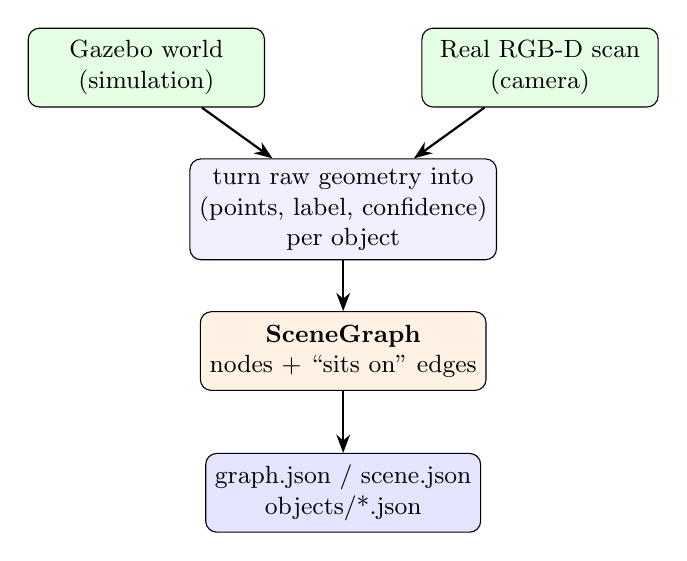
\begin{tikzpicture}
\node[block, fill=green!10] (world)   at (0,0)   {Gazebo world\\(simulation)};
\node[block, fill=green!10] (scan)    at (5,0)   {Real RGB-D scan\\(camera)};
\node[block]                (builder) at (2.5,-1.8) {turn raw geometry into\\(points, label, confidence)\\per object};
\node[block, fill=orange!10](graph)   at (2.5,-3.6) {\textbf{SceneGraph}\\nodes + ``sits on'' edges};
\node[block, fill=blue!10]  (json)    at (2.5,-5.4) {graph.json / scene.json\\objects/*.json};

\draw[arrowline] (world) -- (builder);
\draw[arrowline] (scan)  -- (builder);
\draw[arrowline] (builder) -- (graph);
\draw[arrowline] (graph) -- (json);
\end{tikzpicture}
\end{center}

Two completely different front-ends (a simulator's ground truth, or a neural
network's guesses about a real photo) both reduce to the same simple input:
\emph{a point cloud, a label, and a confidence, for each object}. Everything
after that point is shared code. The rest of this document explains, with
real equations, how each box above is actually computed.

\section{From a cloud of dots to one point: the centroid}

Every object starts out as nothing more than a \textbf{point cloud}: a big
list of 3D points $p_1, p_2, \dots, p_N$, each one $p_i = (x_i, y_i, z_i)$,
roughly tracing the object's surface. The very first question we ask is the
simplest one possible: \emph{where is the middle of all these dots?}

\[
c = \frac{1}{N}\sum_{i=1}^{N} p_i
\]

That's it -- add up every point and divide by how many there are. This is
the \textbf{centroid}, and the code for it
(\texttt{graph\_nodes.py}, \texttt{ObjectNode.\_\_init\_\_}) is literally one
line: \texttt{np.mean(points, axis=0)}.

\begin{center}
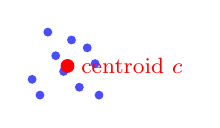
\begin{tikzpicture}[scale=1]
\foreach \x/\y in {0.1/0.3, 0.4/0.6, 0.7/0.2, 0.9/0.5, 0.3/0.9, 0.6/0.8,
                    0.2/0.1, 0.8/0.7, 0.5/0.4, 0.95/0.1}{
  \fill[blue!70] (\x,\y) circle (1.6pt);
}
\fill[red] (0.55,0.47) circle (2.5pt);
\node[red, right] at (0.6,0.47) {\footnotesize centroid $c$};
\end{tikzpicture}
\end{center}

\section{Which way is it facing? Principal Component Analysis (PCA)}

A position alone doesn't tell you which way a banana is pointing. To get an
\textbf{orientation} out of a pile of dots, the code looks for the
\emph{directions the dots are most spread out along} -- the long axis of a
banana is exactly that: the direction where, if you slid a ruler along it,
the points would spread out the most.

\textbf{Step 1 -- centre the points} (so the centroid sits at the origin):
\[
\tilde p_i = p_i - c
\]

\textbf{Step 2 -- measure the spread in every direction at once.} This is
the job of the \textbf{covariance matrix}, a $3\times3$ table:
\[
\Sigma = \frac{1}{N-1}\sum_{i=1}^N \tilde p_i \,\tilde p_i^{\!\top}
\]
Entry $\Sigma_{xx}$ is how spread out the points are along $x$ alone;
$\Sigma_{xy}$ says whether ``being far in $x$'' tends to come together with
``being far in $y$'' too (a tilted blob has large off-diagonal entries).

\textbf{Step 3 -- find the natural axes.} Every covariance matrix has three
special directions $v_1, v_2, v_3$ (\textbf{eigenvectors}) along which it
acts like plain scaling:
\[
\Sigma v_k = \lambda_k v_k
\]
$\lambda_k$ (the \textbf{eigenvalue}) says \emph{how much} spread there is
along $v_k$. Sorting by $\lambda_k$ from largest to smallest gives the
object's natural axes, longest first -- exactly the banana's long axis,
then its two shorter ones.

\textbf{Step 4 -- assemble a rotation matrix.} Stack the three axes as
columns:
\[
R = \begin{bmatrix} v_1 & v_2 & v_3 \end{bmatrix}
\]
One technicality: eigenvectors can come out as a mirror image
($\det R = -1$) instead of a proper rotation ($\det R = +1$). The fix used
in the code is to flip the sign of the last column whenever that happens:
\[
\det R < 0 \;\Longrightarrow\; v_3 \leftarrow -v_3
\]

\textbf{Step 5 -- package it as a pose.} Position and orientation together
become one $4\times4$ \textbf{pose matrix}:
\[
T = \begin{bmatrix} R & c \\ 0\;0\;0 & 1 \end{bmatrix}
\]

\begin{center}
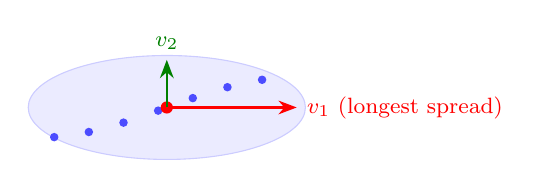
\begin{tikzpicture}[scale=1.1]
\draw[blue!20, fill=blue!8] (0,0) ellipse (1.6 and 0.6);
\foreach \t in {-1.3,-0.9,...,1.3}{
  \fill[blue!70] (\t, {0.35*sin(\t*60)}) circle (1.4pt);
}
\fill[red] (0,0) circle (2pt);
\draw[arrowline, red]   (0,0) -- (1.5,0)   node[right] {\footnotesize $v_1$ (longest spread)};
\draw[arrowline, green!50!black] (0,0) -- (0,0.55) node[above] {\footnotesize $v_2$};
\end{tikzpicture}
\end{center}

\textbf{Analogy:} scatter the object's points on a table and draw the
tightest oval around them. PCA finds that oval's long axis and short axis.

\section{How big is it, and which way is ``up''?}

Position and orientation aren't size. For that, the code asks Open3D for
the \textbf{minimal oriented bounding box} -- the smallest box, allowed to
tilt, that still contains every point (shrink-wrap, instead of a box that
can only line up with $x$/$y$/$z$ and would have to be huge for a tilted
object). That box has its own rotation $R_{\text{box}}$ and an
\textbf{extent} $(e_1, e_2, e_3)$ along its own three axes.

To label those three numbers ``width'', ``depth'', ``height'', the code asks
\emph{which of the box's own axes points closest to straight up}, $e_z =
(0,0,1)$ in the world:
\[
h = \operatorname*{argmax}_{i \in \{1,2,3\}} \big| (R_{\text{box}}^{\top} e_z)_i \big|
\]
That axis $i=h$ becomes the \textbf{height}; the other two, sorted larger
first, become \textbf{width} and \textbf{depth}.

\section{Where do the points come from? Path 1: Gazebo ground truth}

This is the simplest path -- no neural network, every number traced back to
a file on disk.

\subsection{Reading the world file}

\texttt{apartment.world.xacro} expands (via the \texttt{xacro} command) into
plain XML. Every object is one \texttt{<include>} block:
\begin{center}
\texttt{<include><name>hsr\_orange\_02</name><uri>model://hsr\_orange</uri>}\\
\texttt{<pose>4.6 3.9 1.05 0 0 0</pose></include>}
\end{center}
The pose is six numbers $(x, y, z, \phi, \theta, \psi)$ -- a position and
three rotation angles (\textbf{roll}, \textbf{pitch}, \textbf{yaw}).

\subsection{From a shape description to 8 corner points}

Every Gazebo model has its own \texttt{.sdf} file describing its physical
shape as a box, cylinder, sphere, or 3D mesh. For each, the code computes
the 8 corners of that one shape's local bounding box:

\[
\text{box}(w,d,h):\quad \Big(\pm\tfrac{w}{2},\, \pm\tfrac{d}{2},\, \pm\tfrac{h}{2}\Big)
\qquad\quad
\text{sphere}(r):\quad \big(\pm r,\, \pm r,\, \pm r\big)
\]
\[
\text{cylinder}(r,\ell):\quad \Big(\pm r,\, \pm r,\, \pm\tfrac{\ell}{2}\Big)
\]
(all $2\times2\times2=8$ sign combinations of each triple).

\begin{center}
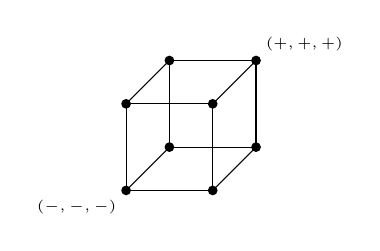
\begin{tikzpicture}[scale=1.1]
\def\a{1}
\draw (0,0) -- (\a,0) -- (\a,\a) -- (0,\a) -- cycle;
\draw (0.5,0.5) -- (\a+0.5,0.5) -- (\a+0.5,\a+0.5) -- (0.5,\a+0.5) -- cycle;
\draw (0,0)--(0.5,0.5);  \draw (\a,0)--(\a+0.5,0.5);
\draw (\a,\a)--(\a+0.5,\a+0.5); \draw (0,\a)--(0.5,\a+0.5);
\foreach \p in {(0,0),(\a,0),(\a,\a),(0,\a),(0.5,0.5),(\a+0.5,0.5),(\a+0.5,\a+0.5),(0.5,\a+0.5)}{
  \fill \p circle (1.6pt);
}
\node[below left] at (0,0) {\tiny$(-,-,-)$};
\node[above right] at (\a+0.5,\a+0.5) {\tiny$(+,+,+)$};
\end{tikzpicture}
\end{center}

A mesh (a \texttt{.dae}/\texttt{.stl} file) instead has its bounds loaded
straight from the file with \texttt{trimesh}, scaled by the SDF's
\texttt{<scale>}; COLLADA files also declare their own unit of measurement,
which gets applied too -- otherwise a mesh authored in decimetres comes out
$10\times$ too big.

\subsection{Composing frames: model, link, and shape}

A shape's corners are defined relative to its own \emph{link}, which is
itself placed relative to its \emph{model}, which is finally placed in the
\emph{world}. Each ``placed relative to'' is one $4\times4$ homogeneous
transform built from a pose $(x,y,z,\phi,\theta,\psi)$:
\[
T(x,y,z,\phi,\theta,\psi) = \begin{bmatrix} R_z(\psi)\,R_y(\theta)\,R_x(\phi) & (x,y,z)^{\top} \\ 0 \; 0 \; 0 & 1 \end{bmatrix}
\]
and frames compose by simple matrix multiplication, left to right, outermost
first:
\[
T_{\text{shape}\to\text{model}} \;=\; T_{\text{model}} \cdot T_{\text{link}} \cdot T_{\text{shape}}
\]

\begin{center}
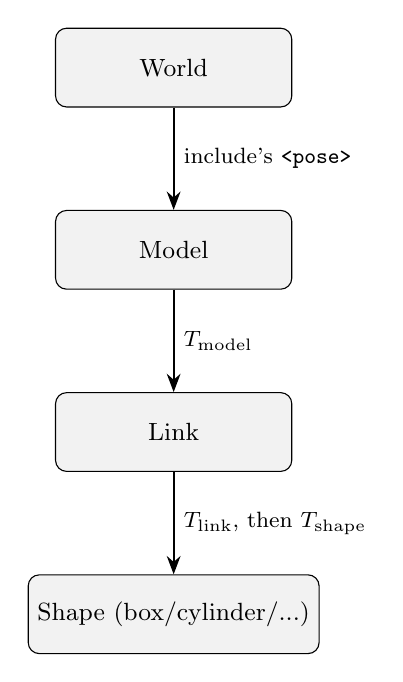
\begin{tikzpicture}[node distance=1.3cm]
\node[block, fill=gray!10] (w) {World};
\node[block, fill=gray!10, below=of w] (m) {Model};
\node[block, fill=gray!10, below=of m] (l) {Link};
\node[block, fill=gray!10, below=of l] (s) {Shape (box/cylinder/...)};
\draw[arrowline] (w) -- (m) node[midway, right] {\footnotesize include's \texttt{<pose>}};
\draw[arrowline] (m) -- (l) node[midway, right] {\footnotesize $T_{\text{model}}$};
\draw[arrowline] (l) -- (s) node[midway, right] {\footnotesize $T_{\text{link}}$, then $T_{\text{shape}}$};
\end{tikzpicture}
\end{center}

Running every shape's 8 corners through this composed transform, then taking
the overall min/max across every link and shape in the model, gives the
model's bounding box \texttt{dims} (width, depth, height) and \texttt{center}
(offset of that box from the model's own origin) -- this is
\texttt{gazebo\_geometry.model\_local\_bbox()}.

\subsection{Sampling a tiny point cloud}

A bounding box isn't a point cloud yet. \texttt{synthesize\_points()} fills
it with an $n\times n\times n$ grid ($n=5$, so 125 points), centred at the
box's local \texttt{center} $(c_x,c_y,c_z)$ with size $(w,d,h)$:
\[
x_i = c_x + \operatorname{linspace}\!\big(-\tfrac{w}{2}, \tfrac{w}{2}, n\big)_i,
\quad \text{(similarly for } y, z \text{)}
\]
then rotates and translates every grid point $p$ by the object's
\emph{world-frame} pose $(R, t)$ from the world file:
\[
p' = R\,p + t
\]
That is the same rotation-matrix recipe as Section 3 ($R = R_z(\psi)R_y(\theta)R_x(\phi)$), just applied here to move a synthetic grid instead of to describe a PCA result.

\section{Where do the points come from? Path 2: a real scan (Mask3D)}

On the real robot, there is no world file -- instead, a neural network
called \textbf{Mask3D} looks at a full-room point cloud and outputs, per
detected object, a binary mask (which points belong to it) and a confidence.
Masks can \emph{overlap} (e.g.\ a table's mask might claim a few points that
really belong to a cup on top of it). The fix: process masks
\textbf{largest first}, each one claiming ownership of its points --
so a \emph{smaller} mask processed later steals its overlapping points back:
\[
\texttt{owner}[p] \;=\; \text{index of the \emph{last} (i.e. smallest) mask that contains } p
\]
After that, every point belongs to exactly one object, and each object's
surviving points become its point cloud -- same input shape as Path 1, just
with a real (not $1.0$) confidence score.

\section{Who is sitting on what? The support score}

Once every object is a node, the code has to decide, for each
\textbf{movable} object, which piece of \textbf{furniture} it's resting on.
The obvious idea -- ``nearest centroid wins'' -- breaks for a shelf unit:
a tall shelf two metres away can have a centroid closer (in 3D) to an apple
than the table directly underneath it, simply because the shelf's centroid
sits up near the apple's own height.

The fix is a \textbf{support score} that measures sideways closeness, but
\emph{penalises} furniture whose centroid floats above the object (since
nothing rests \emph{inside} a shelf above it -- it rests \emph{on top of}
something):
\[
\operatorname{score}(o, f) \;=\; \big\| c_{xy}(o) - c_{xy}(f) \big\|_2 \;+\; \max\!\big(0,\; c_z(f) - c_z(o)\big)
\]
where $c_{xy}$ is just the centroid's $x,y$ part and $c_z$ its height. The
chosen furniture is whichever minimises this score:
\[
f^{\star} = \operatorname*{argmin}_{f \,\in\, \text{furniture}} \operatorname{score}(o, f)
\]

\begin{center}
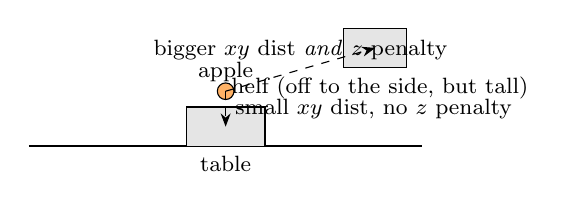
\begin{tikzpicture}[scale=1]
\draw[thick] (-2,0) -- (3,0); % ground
\draw[furn] (0,0) rectangle (1,0.5);     \node[below] at (0.5,0) {\footnotesize table};
\draw[furn] (2,1.0) rectangle (2.8,1.5); \node[below] at (2.4,1.0) {\footnotesize shelf (off to the side, but tall)};
\fill[obj] (0.5,0.7) circle (3pt); \node[above] at (0.5,0.7) {\footnotesize apple};
\draw[dashed, -{Stealth}] (0.5,0.7) -- (0.5,0.25) node[midway, right] {\footnotesize small $xy$ dist, no $z$ penalty};
\draw[dashed, -{Stealth}] (0.5,0.7) -- (2.4,1.25) node[midway, above] {\footnotesize bigger $xy$ dist \emph{and} $z$ penalty};
\end{tikzpicture}
\end{center}

The table wins: its $xy$ distance to the apple is small and, since the
table's centroid sits \emph{below} the apple, the $z$-penalty term is $0$.
The shelf loses on both counts.

\section{Today's upgrade: keeping poses fresh}

Section 5 read every object's pose \emph{once}, from the world file's
static spawn \texttt{<pose>}. That's fine until something actually moves --
the robot bumps a chair, or picks an object up -- after which the
ground-truth scene graph would describe where things \emph{started}, not
where they \emph{are}.

Gazebo already knows the live answer: it publishes every model's current
pose, as a \textbf{quaternion} $(x,y,z,w)$ instead of roll/pitch/yaw (a
quaternion is just a four-number way of writing a rotation that never
suffers from the ``gimbal lock'' problem Euler angles can). To plug a live
pose into the exact same equations as Section 5.4, it first has to be
converted back to $(\phi,\theta,\psi)$:
\[
\phi = \operatorname{atan2}\!\big(2(wx+yz),\; 1-2(x^2+y^2)\big)
\]
\[
\theta = \operatorname{asin}\!\Big(\operatorname{clip}\big(2(wy-zx),\,-1,\,1\big)\Big)
\]
\[
\psi = \operatorname{atan2}\!\big(2(wz+xy),\; 1-2(y^2+z^2)\big)
\]
(\texttt{gazebo\_geometry.quat\_to\_euler()} -- the exact inverse of the
$R = R_z(\psi)R_y(\theta)R_x(\phi)$ recipe from Sections 3 and 5.4.) The
result drops straight into \texttt{synthesize\_points()}'s $p' = Rp + t$
unchanged -- a live pose looks, to the rest of the pipeline, exactly like a
spawn pose. If Gazebo isn't running, the code just falls back to the
world file's static pose, so nothing breaks.

\section{Fast lookups: the KD-tree}

The very last ingredient is a \textbf{KD-tree}: a data structure built once
over every node's centroid, answering ``which node is nearest to this 3D
point?'' in roughly $O(\log N)$ steps instead of checking all $N$ nodes one
by one. It's what lets later code (Section~7's furniture search, or a
mission script asking ``what's near the robot's gripper right now?'') stay
fast even as the scene graph grows.

\section{Glossary}

\begin{center}
\begin{tabular}{@{}p{3.6cm}p{10.5cm}@{}}
\toprule
\textbf{Term} & \textbf{Meaning} \\
\midrule
Point cloud & A set of 3D points, usually tracing an object's surface \\
Centroid & The average position of a set of points \\
Covariance matrix & A $3\times3$ table describing how spread out points are, along and between $x,y,z$ \\
Eigenvector / eigenvalue & A covariance matrix's natural axes, and how much spread lies along each \\
Pose & Position + orientation together, as one $4\times4$ matrix \\
Quaternion & A four-number $(x,y,z,w)$ way of writing a rotation, used by Gazebo's live pose topic \\
(Oriented) bounding box & The smallest, possibly-tilted box containing a set of points \\
KD-tree & A data structure for fast ``nearest point'' queries \\
SDF & Gazebo's XML format describing a model's physical shape \\
Support score & The $xy$-distance-plus-$z$-penalty score deciding which furniture an object rests on \\
\bottomrule
\end{tabular}
\end{center}

\bigskip
\noindent For a code-level, line-by-line walkthrough of the same pipeline,
see \texttt{docs/scene\_graph\_explained.md}. For the full demo-day technical
report (covering the rest of the mission: room clustering, navigation,
detection, grasping), see \texttt{docs/report/scene\_graph\_report.pdf}.

\end{document}
